\documentclass{article}
% To process a .bib file for pdflatex, you should compile your LaTeX document with the sequence: `pdflatex filename.tex`, then run `bibtex filename` (without the .bib extension), followed by two more runs of `pdflatex filename.tex`. This sequence ensures the bibliography is correctly generated and integrated into your document

% if you need to pass options to natbib, use, e.g.:
%  sort&compress option
\PassOptionsToPackage{numbers, compress}{natbib}
% before loading tackling_climate_workshop_style

% ready for submission
\usepackage{tackling_climate_workshop_style}

% to compile a preprint version, e.g., for submission to arXiv, add add the
% [preprint] option:
%     \usepackage[preprint]{tackling_climate_workshop_style}

% to compile a camera-ready version, add the [final] option, e.g.:
%     \usepackage[final]{tackling_climate_workshop_style}

% to avoid loading the natbib package, add option nonatbib:
% \usepackage[nonatbib]{tackling_climate_workshop_style}

\usepackage[utf8]{inputenc} % allow utf-8 input
\usepackage[T1]{fontenc}    % use 8-bit T1 fonts
\usepackage{hyperref}       % hyperlinks
\usepackage{url}            % simple URL typesetting
\usepackage{booktabs}       % professional-quality tables
\usepackage{amsfonts}       % blackboard math symbols
\usepackage{nicefrac}       % compact symbols for 1/2, etc.
\usepackage{microtype}      % microtypography

%%% Packages added by me
\usepackage{caption}
\usepackage{amsmath}
\usepackage{graphicx}
\usepackage{sidecap} % For side captions
\usepackage{ragged2e} % Text alignment (RaggedRight)
\usepackage{colortbl} % For coloring table cells

\title{\textit{Improving Deep Learning-Based Wildfire Smoke Plume Detection with a Multi-Model Ensemble Approach}}
% \title{\textit{A Proposal to Improve Deep Learning-Based Wildfire Smoke Plume Detection with a Multi-Model Ensemble Approach}}

% The \author macro works with any number of authors. There are two commands
% used to separate the names and addresses of multiple authors: \And and \AND.
%
% Using \And between authors leaves it to LaTeX to determine where to break the
% lines. Using \AND forces a line break at that point. So, if LaTeX puts 3 of 4
% authors names on the first line, and the last on the second line, try using
% \AND instead of \And before the third author name.

\author{%
Anonymous Author(s)
  % David S.~Hippocampus\thanks{Use footnote for providing further information
  %   about author (webpage, alternative address)---\emph{not} for acknowledging
  %   funding agencies.} \\
  % Department of Computer Science\\
  % Cranberry-Lemon University\\
  % Pittsburgh, PA 15213 \\
  % \texttt{hippo@cs.cranberry-lemon.edu} \\
  % examples of more authors
  % \And
  % Coauthor \\
  % Affiliation \\
  % Address \\
  % \texttt{email} \\
  % \AND
  % Coauthor \\
  % Affiliation \\
  % Address \\
  % \texttt{email} \\
  % \And
  % Coauthor \\
  % Affiliation \\
  % Address \\
  % \texttt{email} \\
  % \And
  % Coauthor \\
  % Affiliation \\
  % Address \\
  % \texttt{email} \\
}

\begin{document}

\maketitle

\begin{abstract}
With increasing frequency and severity of wildfires, there is an urgent need for wildfire and smoke detection tools that can effectively and rapidly monitor smoke at a large scale. Recent advancements in computer vision have demonstrated the potential of deep learning models to automatically separate high-resolution images into labeled regions for high-accuracy feature detection. However, single-model approaches can struggle with generalization and accuracy in diverse conditions, which is necessary in the operational use of a smoke detection tool. To address these challenges, we propose using an ensemble of deep learning models to produce more accurate annotations of wildfire smoke plumes and their relative density (light, medium, heavy) in satellite imagery. Our preliminary results indicate that ensemble techniques can improve performance compared to using a single model, and that further investigation is needed to optimize the ensemble. This approach aims to provide a more reliable satellite-based tool for real-time monitoring of smoke. This will have numerous downstream impacts, such as aiding fire and hazard management efforts, improving modeling of wildfire behavior and air quality, and ultimately contributing to climate resilience and adaptation strategies.
% Broadly, this will be a valuable tool for air quality and fire hazard management in the face of worsening wildfires.
% This proposal shows that multi-model deep learning ensembles could be used to support fire and hazard management by automating the real-time monitoring of smoke from satellite imagery.  
\end{abstract}

\section{Introduction}
In the last four decades, wildfire activity has increased drastically in the U.S. In fact, the conditions leading to wildfires have been shown to occur more frequently as a direct result of climate change \citep{wildfire-risk}. Wildfires produce particulate emissions, such as smoke and ash, which can be tracked to quantify the impact a fire has beyond its burn area. Satellite observations reveal that the number of days with smoke above the continental U.S. have substantially increased in the last two decades \citep{wildfire-risk}. Futhermore, the human impacts of smoke exposure include increased morbidity and mortality as well as downstream economic costs \citep{health-impacts}.
% may consider omitting sentence 3 or 4 here to be more concise.
% Furthermore, future climate predictions reveal that wildfire-related particulate emissions such as smoke and ash could double in fire-prone areas

Determining causal links between wildfire activity and health impacts in regions distant from the source fire requires accurate large-scale monitoring of wildfire smoke and its movement. An intuitive approach is to utilize satellite-based methods that can monitor evolution of smoke plumes over large areas. However, such methods have yet to provide precise and high-frequency information on smoke density, or are confined to to small case-study regions \citep{Wen2021WildfireSP, canada-smoke-height, autralia-smoke-ml}. 

\section{Background}
\subsection{Current large-scale, satellite-based smoke detection} % 
% \section{Background: current large-scale, satellite-based smoke detection}
The National Oceanic and Atmospheric Administration (NOAA) Geostationary Operational Environmental Satellites (GOES) provide high spatial and temporal resolution imagery of North America \citep{GOESbook}. The NOAA Hazard Mapping System (HMS) Fire and Smoke Product currently relies on expert human analysts to annotate the presence of smoke over North America using GOES imagery \citep{hms}. However, this product is limited by the availability of human analysts and their time, with annotations outputted only once to a few times a day and usually having a delay between smoke occurence and the annotation. Thus, emergency responders may be delayed without real-time smoke conditions, or could miss early detections of fire considering that smoke can obfuscate fire visibility. To address these limitations, we leverage advancements in deep learning to automate the detection of smoke from GOES imagery, using the existing HMS dataset for training. By automating this task, we can enable more frequent detection of smoke plumes, which will aid in active wildfire monitoring and mitigating air quality impacts.
% Deep learning models, particularly encoder-decoder neural networks, have shown promise in automating the semantic segmentation (labelling images on a pixel-wise basis with multiple classes) of high-resolution images \citep{cv-segmentation-review}. 
% ^ Excluding this assuming audience is aware

\subsection{Ensemble techniques}
% \section{Background: Ensemble techniques}
This proposal focuses on enhancing the capability of deep learning models to detect smoke using multi-model ensemble methods. Ensembles, which combine the predictions of multiple models, have been shown to often perform better than a single model in classification tasks \citep{ensemble-ml}. Particularly, utilizing a diverse set of classifiers in an ensemble is important to achieve the improvement in performance \citep{ensemble-diversity}. Furthermore, combining the predictions of multiple independently-trained neural networks can improve generalization and detection accuracy \citep{nn-ensemble,nn-ensemble2, nn-error-ens}. To our knowledge, these ensemble methods have not yet been used for wildfire smoke detection.
% \citep{nn-error-ens} demonstrated the importance of the neural networks having independent errors, or "error diversity" for the ensemble to succeed.
% \citep{nn-error-ens} also provided a mathematical basis (clustering of errors) for designing ensembles that contain error diversity between the models.

\section{Methods} % calling this methods instead of proposed methods since it is methods i've done already and i'm no longer worried about them realizing it is a proposal.
We use the SmokeViz dataset which consists of 183,672 smoke plume samples, each with three spectral channels (C01-C03) of GOES imagery paired with human analyst smoke annotations (pixel-wise labels of smoke density of light, medium, or heavy). The data spans 2018-2024, and we use 2023 for the validation set and 2022 for the test set, with the remaining years used for training. This ensures the testing and validation data are independent of the training data. During validation and testing, we quantify model performance with Intersection over Union (IoU) score, which measures pixel-wise alignment between the model prediction and the ground truth. The IoU metric supports pathways to climate impact since improved IoU score directly relates to more smoke being accurately detected (reducing false detections and increasing true detections) which equips hazard management to appropriately respond to current wildfire and smoke conditions.

We utilize a variety of encoder-decoder architectures designed for semantic segmentation that include different features such as multi-scale fields-of-view and precise boundary detection \citep{dlv3p,PAN,UNetpp}. Additionally, we selected the best-performing single architecture and trained it with 12 seeds to generate different initial random weights. By varying the initialization, the model's parameter space can be searched more fully; ideally, different minima of the loss function will be found. All the models were trained independently for 24 hours on 8 Nvidia P100 GPUs using the Adam optimizer and the binary cross entropy loss function. 
%  contained within the Segmentation Models Pytorch library \citep{semantic}
%  which are important for accurately detecting smoke plumes that can vary in size. 

The ensemble method we are using in this preliminary analysis is an unweighted average of $N$ model outputs (Figure \ref{fig:ensemble_framework}), as used in \citep{nn-ensemble2}. We experimented with the ensemble size in supplementary section \ref{sec:ens-size}, and present results here with $N=8$. We create an architecture-based ensemble and a initialization-based ensemble.

% \subsection{Dataset} 
% \subsection{Metrics} 

% \begin{figure}[h]
%     \centering
%     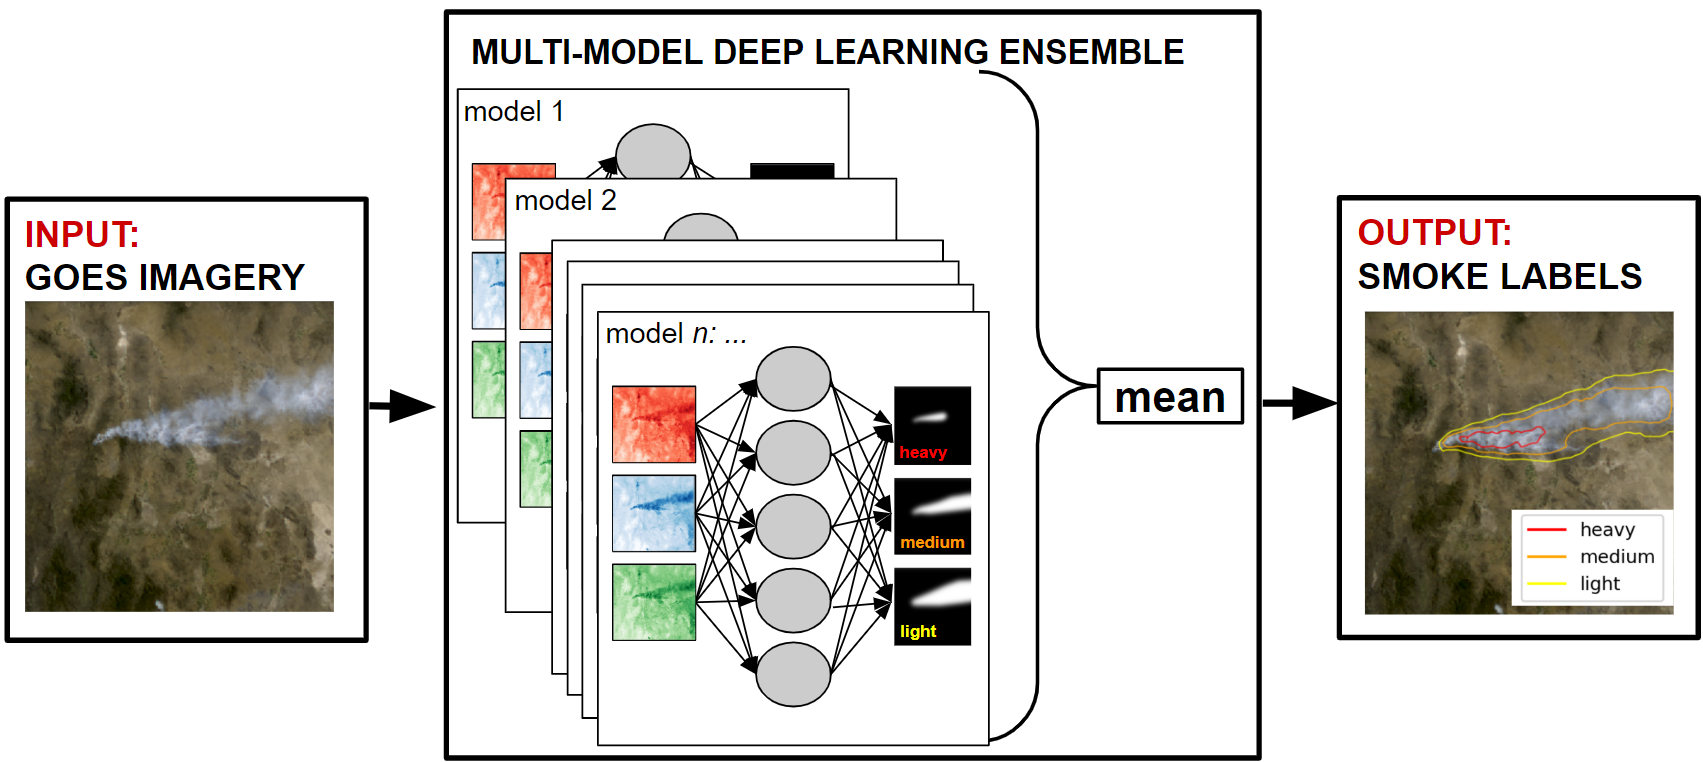
\includegraphics[width=0.7\textwidth]{ensemble_framework.png}
%     \caption{Multi-Model Ensemble Framework. GOES imagery is inputted to N independently-trained models whose output is combined with an unweighted average to produce the ensemble prediction of pixel-wise smoke labels.}
%     \label{fig:ensemble_framework}
% \end{figure}
\begin{SCfigure}[][h]
    \centering
    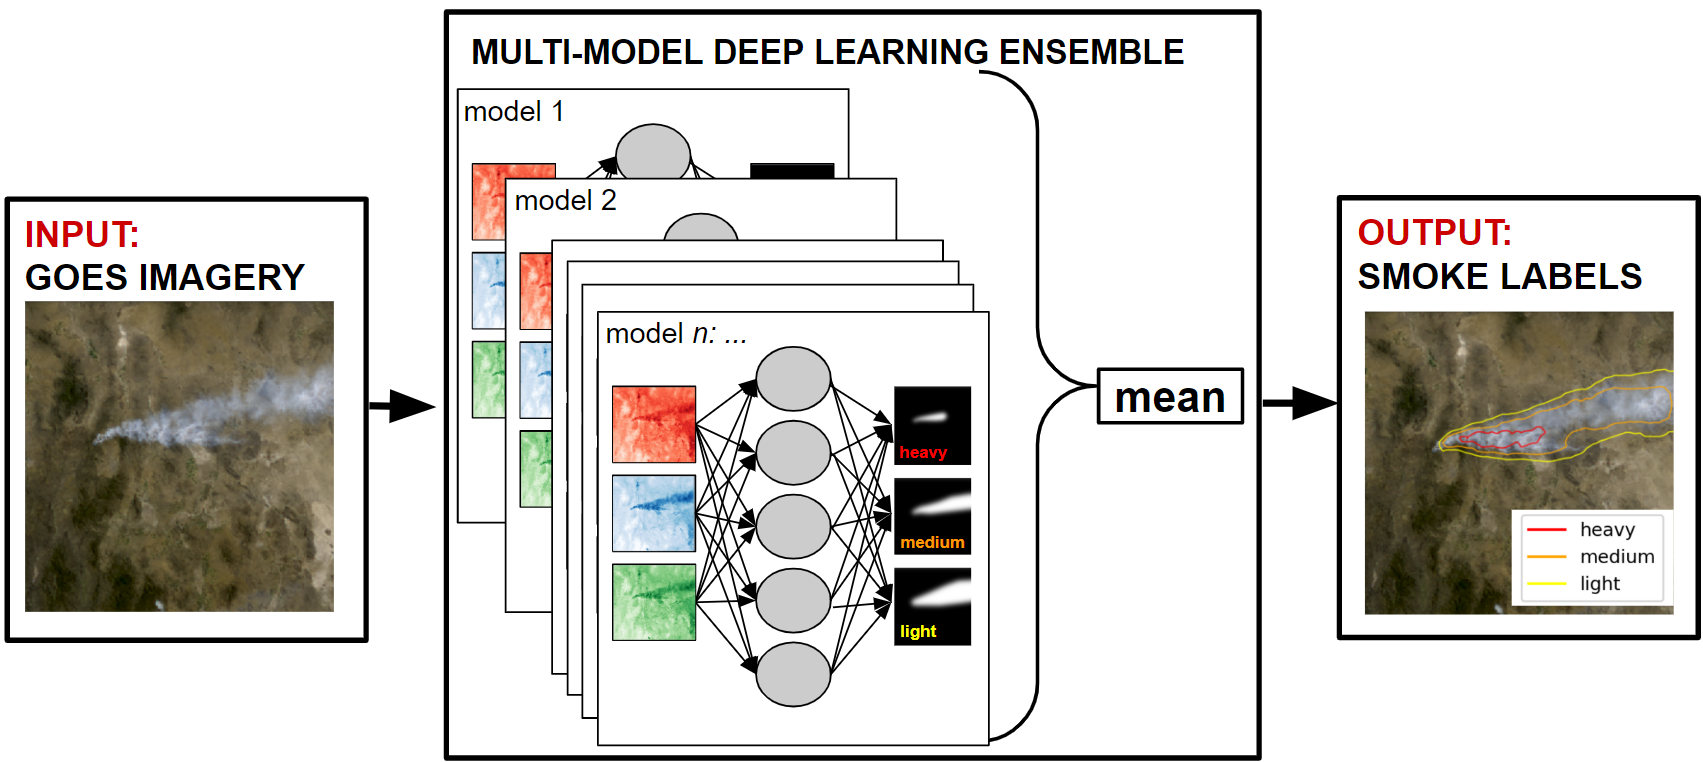
\includegraphics[width=0.7\textwidth]{ensemble_framework.png}
    \caption{\RaggedRight Multi-model ensemble framework. GOES imagery is inputted to $N$ independently-trained models whose output is combined with an unweighted average to produce the ensemble prediction of pixel-wise smoke labels.}
    \label{fig:ensemble_framework}
\end{SCfigure}
\section{Preliminary results}
Table \ref{tab:results} shows the IoU scores on the test set for individual models and ensembles. The ensemble of 8 different architectures outperforms the individual models, with an improvement in all IoU metrics. The ensemble of 8 different initial weights (but the same architecture, PAN) also outperforms the individual models, with a similar improvement in the IoU scores. This improvement is likely due to the different initializations leading to the models searching different parts of the parameter space and thus finding different minima of the loss function. Future work is necessary to reveal the mechanisms behind the ensemble's improvement in performance, as well as how to optimally select models that are included in the ensemble.

Figure \ref{fig:ensemble_panel} shows an example of smoke plume detection from the testing dataset. The ensemble predictions have smoother boundaries than the individual model outputs, making the prediction more comparable to the human analyst-drawn annotations.
\begin{table}[h]
    \centering
    \caption{Test IoU results across heavy, medium and light smoke density and over all densities with single models and ensemble schemes.}
    \label{tab:results}
    \begin{tabular}{llrrr>{\bfseries}r}
        \hline
            &   Heavy &   Medium &   Light &   Overall \\
        \hline
        Single Model: DLV3P \citep{dlv3p} &   0.347 &     0.441 &  0.666 &      0.599  \\
        Single Model: PAN \citep{PAN} &  0.349 &     0.478 &  0.664 &      0.604 \\
        Architecture Ensemble &   0.400 &     0.507 &  0.692 &      0.635 \\ % N=8
        %  Architecture Ensemble (N=12) &  0.400 &     0.504 &  0.686 &      0.630 \\
        Random Initial Weights Ensemble &  0.409 &     0.512 &  0.684 &      0.631 \\% N=8
        %  Random Initial Weights Ensemble (N=12) &   0.409 &     0.515 &  0.690 &      0.635 \\
         \hline
    \end{tabular}
    \end{table}

\begin{figure}[h]
    \centering
    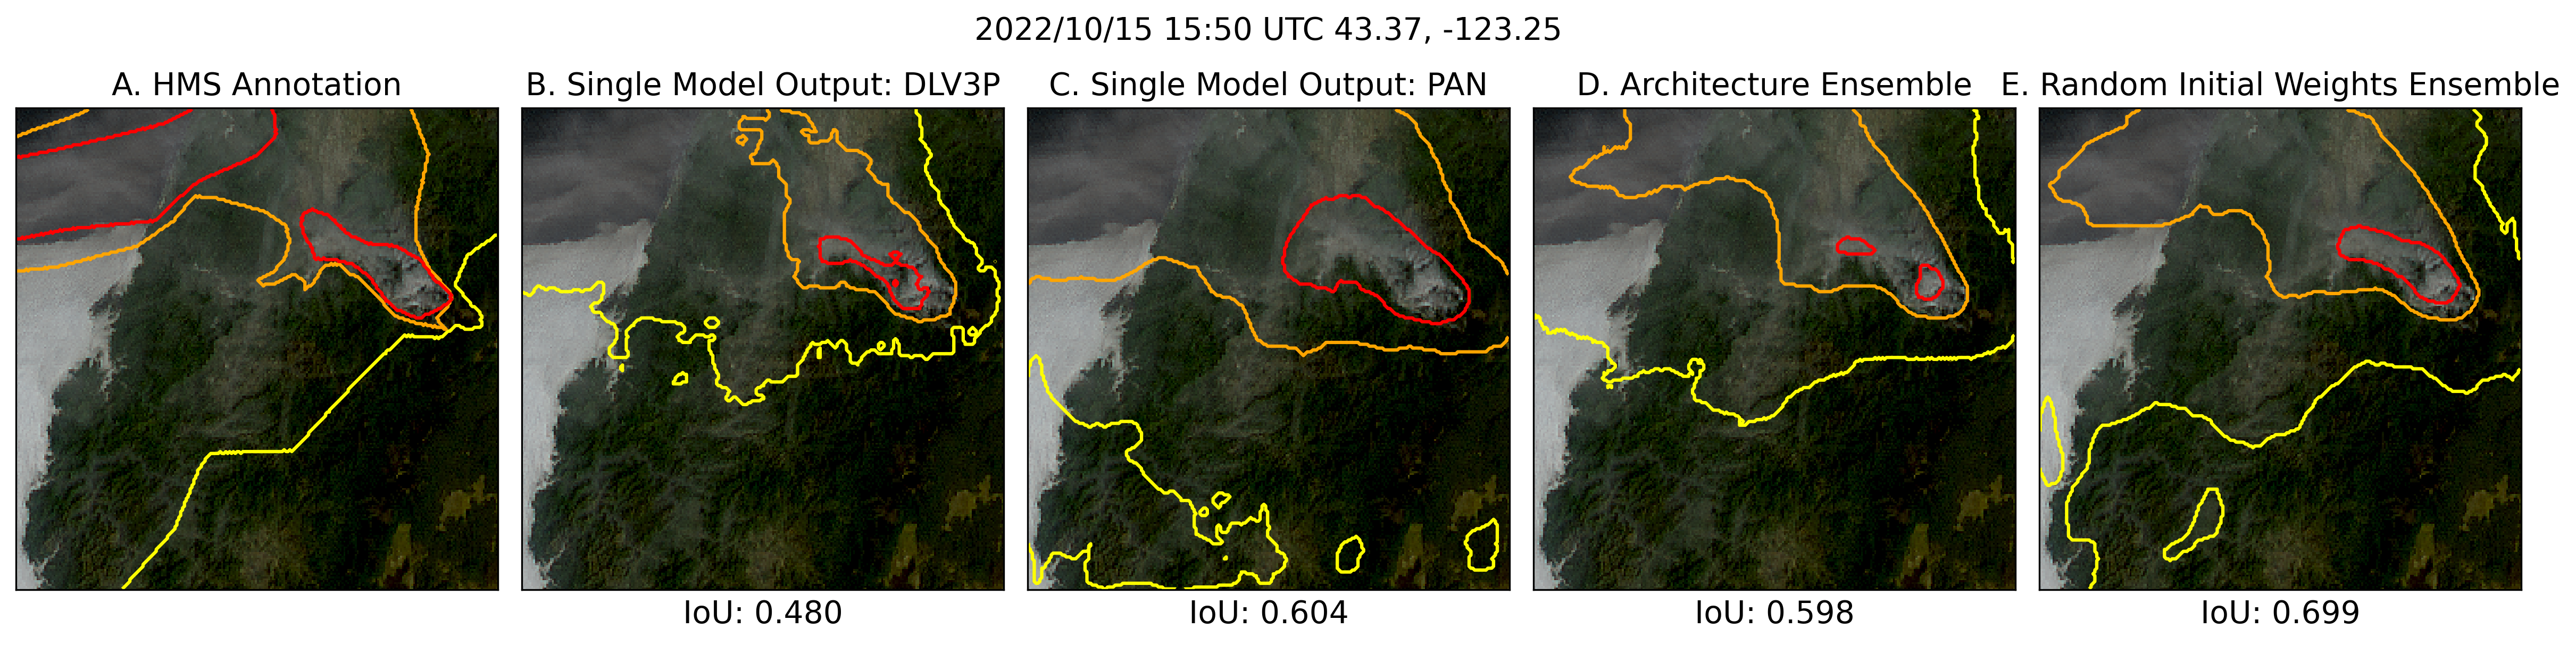
\includegraphics[width=\textwidth]{ensemble_panel_tinypaper.png}
    \caption{Example of smoke plume detection at (43.37$^{\circ}$, -123.25$^{\circ}$) on 2022/10/15 15:50 UTC. Red, orange, and yellow contours represent heavy, medium and light density smoke annotation/prediction, respectively. (A) displays the ground truth annotation; (B-C) show the predictions of two individual models; (D) shows the prediction of the architecture-based ensemble; (E) shows the prediction of an ensemble made with models initialized with different random weights.}
    % is it intuitive how I listed the panels as (A), (B-C)...
    \label{fig:ensemble_panel}
\end{figure}
\section{Limitations and future work} This proposal explores two schemes for building ensembles of deep learning models that both improve on testing set IoU and smooth annotation boundaries. However, further investigation is required to give insight on how the ensemble reduces error and improves generalizability and what the optimal ensemble size and type are. One area to explore is "stacking", where an optimized meta-model is used to combine multi-model outputs \cite{pm2.5-stack, rainfall-stack}. Furthermore, future work will utilize the multi-model ensemble to quantify uncertainty in smoke annotations, enabling users like wildfire response teams and environmental agencies to assess the reliability of detections in real time. 

\section{Pathways to climate impact} These ensemble techniques can be used to aid fire and hazard management by automating the monitoring of smoke in real-time from satellite imagery with smooth and accurate smoke annotations. This will improve prediction of wildfire movement and air quality impacts, ultimately supporting climate resilience and adaptation strategies.  

\newpage
\bibliographystyle{unsrt}
\bibliography{references} 

\section{Supplementary Material}
\subsection{Data and Code Availability} The code for this work is available at \url{https://github.com/anonymous-ensemble-smoke/ensemble-AI-smoke-detection/tree/main}. The dataset can be accessed at \url{https://noaa-gsl-experimental-pds.s3.amazonaws.com/index.html#SmokeViz/}.

\subsection{Ensemble Size Analysis}\label{sec:ens-size} 
Figure \ref{fig:ensemble_size_plot} shows the IoU performance over all smoke densities as a function of ensemble size, $N$, for the two ensemble schemes. The ensemble with different initial weights generally improves as models are added to the ensemble. The ensemble of different architectures improves with more models up to 8 models, but then decreased in IoU with more models added to the ensemble. This decrease in performance could be due to the additional architectures not having enough variation in model bias to improve ensemble performance. Future work will aim to clarify exactly how different ensemble sizes behave and reduce error. 

An additional example from the test data set is shown in Figure \ref{fig:smoothing_ex}, where the individual model output has jagged boundaries and the ensemble outputs smooth over these edges. We see a peak in performance at $N=8$ in this sample where the $N=8$ ensemble has the highest IoU score, and the smoothing does not seem to improve in the $N=12$ ensemble output. This sample supports the proposed idea that ensemble deep learning can smooth over rough edges in semantic segmentation, and warrants further investigation for the optimal ensemble and how to use the multi-model approach to quantify uncertainty. 
\begin{SCfigure}[][h]
    \centering
    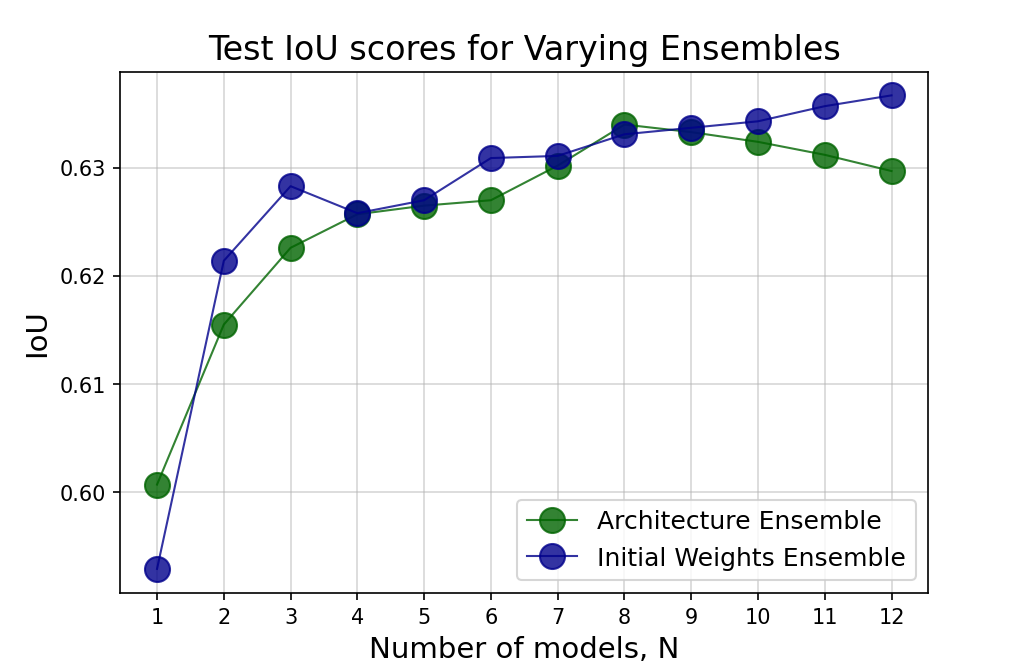
\includegraphics[width=0.70\textwidth]{ensemble_size_plot.png}
    \caption{\RaggedRight Overall IoU as a function of $N$ for two ensemble design schemes: random initial weights (blue) and architecure-based (red).}
    \label{fig:ensemble_size_plot}
\end{SCfigure}

\begin{figure}[h]
    \centering
    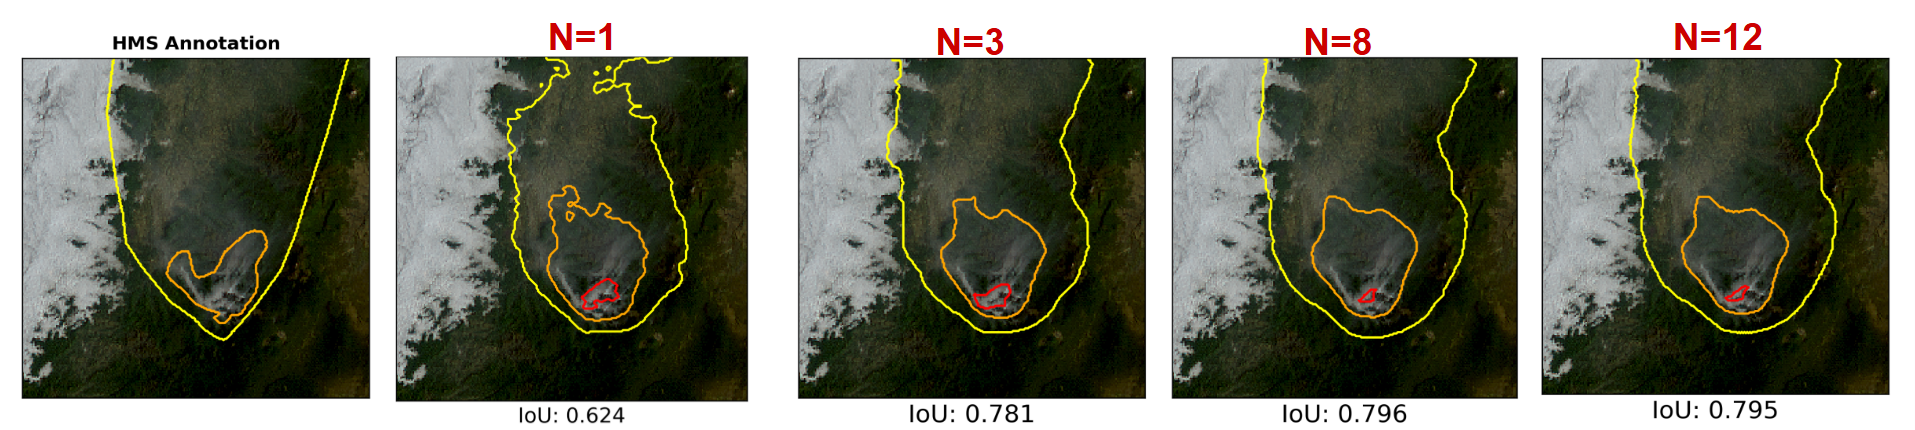
\includegraphics[width=\textwidth]{smoothing_ex.png}
    \caption{Example of smoke plume detection at (44.24, -122.74) on 2022/09/27 15:30 UTC. Red contours outline the heavy density smoke, orange contours outline the medium density smoke, and yellow contours outline the light density smoke annotations. The first panel displays the ground truth HMS annotation; the second panel is the individual model output of DLV3P; the following panels the prediction of an architecture-based ensemble as it increases in size, $N$.}
    \label{fig:smoothing_ex}
\end{figure}

\subsection{Intersection Over Union (IoU) formula}
Equation \ref{overall_iou} provides a mathematical formula for IoU, where $y_{i}$ represents the ground truth and $y^*_{i}$ represents the model's prediction.
\begin{equation} \label{overall_iou}
    \text{IoU}_{\text{overall}} = {\sum\limits_{i=\text{light}}^{\text{heavy}}|y_{i}\cap y^*_{i}|} \div {\sum\limits_{i=\text{light}}^{\text{heavy}}|y_{i}|\cup|y^*_{i}|}
\end{equation}
%  why the architecture-based ensemble decreases in performance after 8 models,


% The \LaTeX{} style file contains three optional arguments: \verb+final+, which
% creates a camera-ready copy, \verb+preprint+, which creates a preprint for
% submission to, e.g., arXiv, and \verb+nonatbib+, which will not load the
% \verb+natbib+ package for you in case of package clash.

% \paragraph{Paragraphs}

% In \LaTeX{} there is also a \verb+\paragraph+ command available, which sets the heading in bold, flush left, and inline with the text, with the heading followed by 1\,em of space. If using this style option in a \verb+docx+ file, please follow these instructions accordingly.
% would using the paragraph command save space?

% Use unnumbered first-level heading for the references. Q: what does  this mean?

% \subsection{Citations within the text}

% Citations within the text should be numbered consecutively.  The corresponding number is to appear enclosed in square brackets, such as [1] or [2]-[5].  The corresponding references are to be listed in the same order at the end of the paper, in the \textbf{References} section. (Note: the standard
% \textsc{Bib\TeX} style \texttt{unsrt} produces this.) As to the format of the references themselves, any standard reference style is acceptable, as long as it is used consistently.

% When using the \LaTeX{} template, the \verb+natbib+ package will be loaded for you by default.  Citations may be author/year or numeric, as long as you maintain internal consistency.

% For \LaTeX{} use, note that the documentation for \verb+natbib+ may be found at
% \begin{center}
%   \url{http://mirrors.ctan.org/macros/latex/contrib/natbib/natnotes.pdf}
% \end{center}
% Of note is the command \verb+\citet+, which produces citations appropriate for
% use in inline text.  For example,
% \begin{verbatim}
%    \citet{hasselmo} investigated\dots
% \end{verbatim}
% produces
% \begin{quote}
%   Hasselmo, et al.\ (1995) investigated\dots
% \end{quote}

% If you wish to load the \verb+natbib+ package with options, you may add the
% following before loading the \verb+neurips_2020+ package:
% \begin{verbatim}
%    \PassOptionsToPackage{options}{natbib}
% \end{verbatim}

% If \verb+natbib+ clashes with another package you load, you can add the optional
% argument \verb+nonatbib+ when loading the style file:
% \begin{verbatim}
%    \usepackage[nonatbib]{tackling_climate_workshop_style}
% \end{verbatim}
\end{document}